% =====================================================================
%  SUPERVISOR BRIEF -- four follow-on papers on two pages.
%
%  Self-contained: no \input, no bibliography, no external files.
%  Compile with pdfLaTeX on Overleaf (any TeX Live 2020 or later).
% =====================================================================
\PassOptionsToPackage{table}{xcolor}
\documentclass[10pt,a4paper]{article}
\usepackage[T1]{fontenc}
\usepackage[utf8]{inputenc}
\usepackage{mathptmx}
\usepackage[a4paper,top=12mm,bottom=13mm,left=14mm,right=14mm]{geometry}
\usepackage{amsmath,amssymb}
\usepackage{xcolor}
\usepackage{tabularx,booktabs,array}
\usepackage{enumitem}
\usepackage[most]{tcolorbox}
\usepackage{tikz}
\usetikzlibrary{arrows.meta,positioning,calc}
\usepackage{microtype}
\usepackage[hidelinks]{hyperref}

\pagestyle{empty}
\setlength{\parindent}{0pt}
\setlength{\parskip}{2pt}

% ---- palette (matches the parent manuscript) -------------------------
\definecolor{netcol}{RGB}{31,78,121}
\definecolor{autocol}{RGB}{18,120,90}
\definecolor{bridgecol}{RGB}{176,96,0}
\definecolor{accent}{RGB}{140,20,20}
\definecolor{soft}{RGB}{244,246,249}

\newcolumntype{Y}{>{\raggedright\arraybackslash}X}
\newcolumntype{P}[1]{>{\raggedright\arraybackslash}p{#1}}
\setlist{nosep,leftmargin=1.1em,topsep=1pt}

% ---- a paper card ----------------------------------------------------
% #1 colour, #2 label, #3 title, #4 venue line
\newtcolorbox{card}[4]{%
  enhanced, colback=white, colframe=#1, boxrule=0.6pt, arc=1.5pt,
  left=5pt, right=5pt, top=3pt, bottom=3pt, before skip=5pt, after skip=2pt,
  title={\textbf{#2}\quad #3\hfill\normalfont\small #4},
  coltitle=white, colbacktitle=#1, fonttitle=\normalsize,
  toptitle=1.5pt, bottomtitle=1.5pt}

\newcommand{\hd}[1]{\textcolor{netcol}{\textbf{#1}}\enspace}
\newcommand{\prov}[1]{\textsc{\footnotesize[#1]}}

\begin{document}
\small

% =====================================================================
%  HEADER
% =====================================================================
\begin{tcolorbox}[enhanced, colback=soft, colframe=soft, arc=0pt,
                  left=6pt, right=6pt, top=4pt, bottom=4pt, before skip=0pt]
{\Large\bfseries\color{netcol} Four Follow-on Papers from \emph{From Wire to Flight}}\par
\vspace{1pt}
{\normalsize Research programme brief for supervisors
 \enspace$\cdot$\enspace Roger Nick Anaedevha
 \enspace$\cdot$\enspace RobustUAVs.ai
 \enspace$\cdot$\enspace 1 October 2026}\par
\vspace{2pt}
\footnotesize Parent manuscript: \emph{From Wire to Flight: A Conditional
Mission-Completion Guarantee for UAVs} (with M.~Conti and F.~Cor\`o; targeted at
IEEE S\&P~2027). Papers~I--II grow from its stated limitations; Papers~III--IV
from the CERTIFLIGHT MSCA proposal.
\end{tcolorbox}

% =====================================================================
%  PROGRAMME LOGIC
% =====================================================================
\hd{One chain, four papers.} The parent paper proves a chain from a network
detector's threshold $\theta$ to a certified floor on the mission-completion
rate. Each follow-on paper attacks a different link, so the four do not
overlap and each cites the others.

\vspace{1pt}
\begin{center}
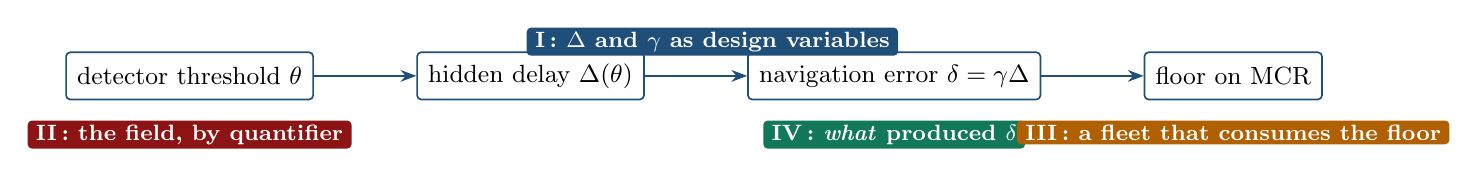
\begin{tikzpicture}[
  node distance=13mm,
  box/.style={draw=netcol, fill=white, rounded corners=1.5pt, line width=0.6pt,
              minimum height=6mm, inner xsep=4pt, font=\small},
  pap/.style={fill=#1, text=white, rounded corners=1.5pt, font=\footnotesize\bfseries,
              inner xsep=3pt, inner ysep=1.5pt},
  arr/.style={-{Stealth[length=2mm]}, line width=0.6pt, draw=netcol}]
  \node[box] (th) {detector threshold $\theta$};
  \node[box, right=of th] (De) {hidden delay $\Delta(\theta)$};
  \node[box, right=of De] (de) {navigation error $\delta=\gamma\Delta$};
  \node[box, right=of de] (mc) {floor on $\mathrm{MCR}$};
  \draw[arr] (th) -- (De); \draw[arr] (De) -- (de); \draw[arr] (de) -- (mc);
  \node[pap=netcol,    above=2.5mm of $(De)!0.5!(de)$] {I\,: $\Delta$ and $\gamma$ as design variables};
  \node[pap=autocol,   below=2.5mm of de] {IV\,: \emph{what} produced $\delta$};
  \node[pap=bridgecol, below=2.5mm of mc] {III\,: a fleet that consumes the floor};
  \node[pap=accent,    below=2.5mm of th] {II\,: the field, by quantifier};
\end{tikzpicture}
\end{center}
\vspace{-3pt}

% =====================================================================
%  PAPER I
% =====================================================================
\begin{card}{netcol}{Paper I}
  {What Authenticity Costs in Metres: A Certified Budget for Cryptography and
   Sensing in UAV Navigation}
  {}
\textbf{Venue:} IEEE S\&P, main track \enspace$\cdot$\enspace
\textbf{Source:} merges proposals P1 (alternative PNT) and P2 (post-quantum
signing) \enspace$\cdot$\enspace \textbf{Effort:} $\approx$5 months

\begin{tabularx}{\linewidth}{@{}P{0.485\linewidth}@{\hspace{0.03\linewidth}}P{0.485\linewidth}@{}}
\hd{Core innovation} Authentication appears on \emph{both} sides of the
certified budget $\rho=(\Delta+\Delta_{\mathrm{auth}})\,\gamma\,e^{LT_c}\le m$.
Authenticating a navigation source lowers $\gamma$ (it can be trusted);
authenticating a message raises $\Delta$ (signing takes time). The certificate
decides the net sign:
\[
\text{authentication pays}\iff
\Delta_{\mathrm{auth}}<\Delta(\theta)\Big(\tfrac{\gamma_u}{\gamma_a}-1\Big).
\]
Two further results: a tighter detector makes authentication \emph{more
affordable but less beneficial}; and signatures protect against delay only via
a freshness check whose clock is itself GNSS-disciplined.
&
\hd{Approach} Measure $\gamma$ for three navigation sources (GNSS done;
inertial-only from flight logs already on disk; visual--inertial). Measure the
cost of five schemes (HMAC-SHA256, Ed25519, ML-DSA-44, SLH-DSA, TESLA) on an
STM32H7-class board and a companion computer, over classic CAN, CAN-FD and
MAVLink~2; validate fragmentation against real bus timing (HCRL UAVCAN). Map
the crossover per (transport, scheme, source).

\hd{Expected results} From the parent's constants \prov{derived}: an
authentication budget of $0.445$\,s at $m{=}5$\,m, $1.39$\,s at $10$\,m, and
\emph{none} at $2$\,m. Prediction \prov{estimate}: ML-DSA-44 costs
${\approx}45$\,ms per message --- affordable --- yet saturates a classic CAN bus
near $22$ msg/s. \emph{The cost is a cliff, not a slope.}
\end{tabularx}
\textbf{Status:} budget arithmetic done; inertial $\gamma$ $\approx$1 week.
\textbf{Main risk:} hardware access (fallback: pinned ARM, tagged as such).
\end{card}

% =====================================================================
%  PAPER II
% =====================================================================
\begin{card}{accent}{Paper II}
  {SoK: The Quantifier Gap Between Certified Robustness and Airworthiness
   Assurance}
  {}
\textbf{Venue:} IEEE S\&P, SoK track (fallback: DASC / ACM CSUR)
\enspace$\cdot$\enspace \textbf{Source:} broadens P3 \enspace$\cdot$\enspace
\textbf{Effort:} $\approx$3 months, no measurement

\begin{tabularx}{\linewidth}{@{}P{0.485\linewidth}@{\hspace{0.03\linewidth}}P{0.485\linewidth}@{}}
\hd{Core innovation} Certified guarantees and aviation assurance objectives both
carry a \emph{quantifier}: per input, per trajectory, per operation, or per
population. Evidence transfers only when the guarantee's quantifier covers the
objective's, or through a \emph{lift} (a dynamics bound, a concentration
argument, a runtime monitor) whose assumption is itself an assurance obligation.
The parent paper is a worked instance: three lifts, three stated conditions.
&
\hd{Approach} Systematic review 2017--2026 across security, ML, verification and
avionics venues; stated inclusion criteria; snowballing to saturation; two
independent coders with Cohen's $\kappa$. Code SORA~2.5, EASA learning-assurance
and ED-324 objectives on the same fields; join the two into a transfer table.

\hd{Expected results} The transfer table (discharge / evidence via lift /
category error); an accounting of lifts as obligations; a ranked research
agenda; a SORA Annex~A evidence generator that keeps every assumption visible.
\end{tabularx}
\textbf{Status:} framework defined; corpus \emph{not yet collected} (expected
80--150 papers). \textbf{Main risk:} a thin or biased corpus.
\end{card}

% =====================================================================
%  PAPER III
% =====================================================================
\begin{card}{bridgecol}{Paper III}
  {Certificates as Constraints: Feasibility-Preserving Multi-Agent RL for
   Swarms Whose Guarantees Degrade}
  {}
\textbf{Venue:} NeurIPS, main track \enspace$\cdot$\enspace
\textbf{Source:} CERTIFLIGHT O3, theorems T3--T4 (WP4) \enspace$\cdot$\enspace
\textbf{Effort:} $\approx$4--5 months

\begin{tabularx}{\linewidth}{@{}P{0.485\linewidth}@{\hspace{0.03\linewidth}}P{0.485\linewidth}@{}}
\hd{Core innovation} Safe RL offers constraints satisfied \emph{in expectation}
(Lagrangian, CPO) or \emph{pointwise} from a hand-set margin (shields, barrier
functions). Here the constraint set is the output of a formal certificate that
\emph{moves over time}: agent $i$ may hold task $\tau$ only while its certified
radius $R_i(t)\ge R_{\min}(\tau)$. Because qualifying radii are nested,
feasibility and robustness collapse to linear-time checks: full coverage
survives any $k$ certificate collapses iff $n(\rho_j)\ge j+k$ for all $j$.
&
\hd{Approach} A constrained MDP over the existing fleet simulator; a projection
layer onto the certified-feasible set, active during training as well as
deployment. Baselines: MAPPO, PPO-Lagrangian, CPO, shielded MADDPG, QMIX, and a
fixed-margin allocator, each with and without the projection layer.

\hd{Expected results} Zero pointwise violations \emph{during training} (versus
in-expectation satisfaction for Lagrangian baselines); a measured
coverage-versus-degradation curve against the proved bound; an honest
scalability ceiling.
\end{tabularx}
\textbf{Status:} four propositions proved; the two combinatorial ones agree with
a brute-force oracle on 3000/3000 random instances. RL study not yet run;
simulator capped at 12 agents. \textbf{Reviewer question to pre-empt:} with an
exact per-step check, learning must earn its place through travel time,
switching cost and forecastable degradation --- the study must beat a greedy
oracle, not only RL baselines.
\end{card}

% =====================================================================
%  PAPER IV
% =====================================================================
\begin{card}{autocol}{Paper IV}
  {When the Attacker Is Indistinguishable from the Weather: A Cross-Layer
   Benchmark and a Unified Perturbation Budget}
  {}
\textbf{Venue:} USENIX Security \enspace$\cdot$\enspace
\textbf{Source:} CERTIFLIGHT O1--O2, theorems T1--T2 (WP2--WP3)
\enspace$\cdot$\enspace \textbf{Effort:} $\approx$5--6 months

\begin{tabularx}{\linewidth}{@{}P{0.485\linewidth}@{\hspace{0.03\linewidth}}P{0.485\linewidth}@{}}
\hd{Core innovation} From the navigation input alone, shaped interference, a
sensor fault and a gust are indistinguishable --- so a certificate sound only
against a declared attack model is unsound against an adversary who resembles
the weather. The budget must therefore be source-agnostic:
$\delta_{\mathrm{tot}}=\delta_{\mathrm{net}}(\theta)\oplus\delta_{\mathrm{gnss}}
\oplus\delta_{\mathrm{fault}}\oplus\delta_{\mathrm{env}}$, combining
worst-case, stochastic and bounded-unknown sources in one certified floor.
&
\hd{Approach} Add fault and environment terms to the certificate engine;
characterise the union bound's slack as a dependence-uncertainty
(Makarov/VaR-aggregation) gap; release the cross-layer benchmark whose records
carry an enforced provenance flag; check soundness at every operating point
across seeds with Holm correction.

\hd{Expected results} Evidence that the composed floor holds where a
signature-tuned detector alone fails silently; a measured union-bound gap; a
public benchmark positioned to become a community evaluation substrate.
\end{tabularx}
\textbf{Status:} six-corpus ingest, certificate engine, residual-budget lemma,
provenance flags in hand. \textbf{Open:} the Makarov reduction is \emph{to be
proved} (fallback: the sound union bound, gap reported empirically).
\end{card}

% =====================================================================
%  AT A GLANCE
% =====================================================================
\vspace{4pt}
{\large\bfseries\color{netcol} At a glance}\par\vspace{2pt}
\renewcommand{\arraystretch}{1.18}
\begin{tabularx}{\linewidth}{@{}P{0.07\linewidth}P{0.13\linewidth}YP{0.19\linewidth}P{0.19\linewidth}P{0.07\linewidth}@{}}
\toprule
\textbf{Paper} & \textbf{Venue} & \textbf{Headline claim, one line} &
\textbf{In hand} & \textbf{Biggest open item} & \textbf{Effort} \\
\midrule
I   & S\&P main &
Authentication is both a credit and a debit on one certified budget; a
closed-form crossover decides which wins. &
derived budget; $\gamma$ for GNSS; flight logs on disk &
benchmark hardware & 5 mo \\
II  & S\&P SoK &
Guarantees and assurance objectives transfer only when their quantifiers
match, or through a lift that is itself an obligation. &
framework; coding scheme &
literature corpus & 3 mo \\
III & NeurIPS &
A formal certificate can serve as a time-varying, pointwise constraint, with
feasibility kept during learning. &
four propositions; 3000/3000 oracle check &
RL study; simulator $>$12 agents & 4--5 mo \\
IV  & USENIX Sec. &
Because attacks, faults and gusts are indistinguishable at the input, only a
source-agnostic budget is a security guarantee. &
six-corpus ingest; engine; provenance flags &
Makarov reduction; benchmark release & 5--6 mo \\
\bottomrule
\end{tabularx}

% =====================================================================
%  TIMELINE
% =====================================================================
\vspace{6pt}
{\large\bfseries\color{netcol} Indicative timeline}
\enspace{\footnotesize\color{black!65}(months from approval; planning estimate, not a commitment)}\par\vspace{2pt}
\newcommand{\cellOn}[1]{\cellcolor{#1!70}}
\newcommand{\cellWr}[1]{\cellcolor{#1!30}}
\setlength{\tabcolsep}{3pt}
\begin{tabularx}{\linewidth}{@{}P{0.09\linewidth}*{8}{>{\centering\arraybackslash}X}@{}}
\toprule
 & M1 & M2 & M3 & M4 & M5 & M6 & M7 & M8 \\
\midrule
II  & \cellOn{accent} & \cellOn{accent} & \cellWr{accent} &  &  &  &  &  \\
I   & \cellOn{netcol} & \cellOn{netcol} & \cellOn{netcol} & \cellOn{netcol} & \cellWr{netcol} &  &  &  \\
IV  & \cellOn{autocol} & \cellOn{autocol} & \cellOn{autocol} & \cellOn{autocol} & \cellOn{autocol} & \cellWr{autocol} &  &  \\
III &  &  & \cellOn{bridgecol} & \cellOn{bridgecol} & \cellOn{bridgecol} & \cellOn{bridgecol} & \cellWr{bridgecol} &  \\
\bottomrule
\end{tabularx}
\vspace{1pt}
{\footnotesize Dark: research and experiments. Light: writing and submission.
Paper~II's first two months are search and coding; Paper~I front-loads the
inertial-only $\gamma$ (about one week, data already on disk); Paper~III starts
once I and IV are producing certified radii, though its theory is already done.}

% =====================================================================
%  ORDER AND DECISIONS
% =====================================================================
\vspace{6pt}
\begin{tabularx}{\linewidth}{@{}P{0.30\linewidth}@{\hspace{0.03\linewidth}}Y@{}}
\hd{Proposed order}
\begin{enumerate}[leftmargin=1.3em]
\item \textbf{II} first: cheapest, no hardware, and it fixes the vocabulary the
  other three cite.
\item \textbf{I} and \textbf{IV} in parallel: they share the certificate engine
  but need different hardware and data.
\item \textbf{III} last: it consumes the certified radii that I and IV produce.
\end{enumerate}
&
\hd{Decisions requested from supervisors}
\begin{enumerate}[leftmargin=1.3em]
\item Approve the four-paper split and the venue for each.
\item Paper~I: access to a Pixhawk-class board and a CAN/CAN-FD interface,
  or agreement to the pinned-ARM fallback.
\item Paper~II: a second coder for the literature review (needed for
  Cohen's $\kappa$).
\item Paper~III: GPU allocation on the group cluster, and agreement to extend
  the simulator beyond 12 agents.
\item Lead and co-author arrangement for each paper.
\end{enumerate}
\end{tabularx}

% =====================================================================
%  HONESTY NOTE
% =====================================================================
\vspace{6pt}
\begin{tcolorbox}[enhanced, colback=soft, colframe=soft, arc=0pt, left=6pt,
                  right=6pt, top=3pt, bottom=3pt]
\footnotesize
\textbf{\color{accent}What is established and what is not.}
Parent-paper values are \emph{measured}: hidden delay saturates at
$4.84$\,s over $15{,}392$ relay hops; $\gamma\le1.625$\,m/s over $674$
post-onset samples, varying $6.1\times$ with conditions, calibrated in hover on
one airframe. Paper~I's budget figures are \prov{derived} from those constants;
its CAN-bus figures are an \prov{estimate} from an assumed frame model, to be
replaced by measurement. Paper~III's propositions are proved and checked
against brute force; its learning results do not yet exist. Paper~IV's Makarov
reduction is a claim to prove, with the sound union bound as fallback.
Paper~II's corpus has not been collected. No item on these two pages is
presented as a result before it exists.
\end{tcolorbox}

\end{document}
